\subsubsection{Эйлерова характеристика многообразий}

\begin{remark}
    Хоть теорема и доказана, но может возникнуть ситуация, когда разными словами представлены одни и те же многообразия. Для проверки того, что доказанная теорема действительно является теоремой классификации, нужно использовать характеристики, которые одинаковы для гомеоморфных многообразий.
\end{remark}

\begin{definition}
    Для двумерного многообразия $X$ с данной триангуляцией число
    \[B - P + \Gamma = \chi(X)\]
    называется \textit{эйлеровой характеристикой $X$}, где $B$ — число вершин триангуляции, $P$ — число рёбер триангуляции, $\Gamma$ — число треугольников триангуляции.
\end{definition} 

\begin{theorem}
    Число $\chi(X)$ не зависит от триангуляции.
\end{theorem} 
\begin{proof}
    Полноценное доказательство слишком затруднительно. Нужно доказать, что для любых двух триангуляций многообразия число $B - P + \Gamma$ одинаково. Для простых триангуляций, подобных тем, что изображены на рисунке \ref{fig:c11.1}, доказать несложно — достаточно рассмотреть рёбра обеих триангуляций и подразбить, если требуется, треугольники на более мелкие (измельчить триангуляцию) так, чтобы новая триангуляция была измельчением уже существующих. Однако если рёбра триангуляций — произвольные кривые (например, $\sin{\frac{1}x})$), такое рассуждение не годится.

    \begin{figure}[ht]
        \centering
        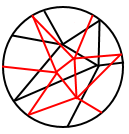
\includegraphics[scale=0.7]{images/c11.1.png}
        \caption{Различные триангуляции многообразия.}
        \label{fig:c11.1}
    \end{figure}
\end{proof} 

Если эйлерова характеристика двух многообразий различна, то эти многообразия не гомеоморфны. Вычислим эйлерову характеристику для многообразий из списка в теореме.

Для сферы $\chi(\mathbb{S}^2) = 2$ (мы уже вычисляли эйлерову характеристику сферы, так как рёбра триангуляции можно рассматривать как граф на сфере). В качестве поверхности, гомеоморфной сфере, можно рассмотреть произвольный выпуклый многогранник, например, тетраэдр.

Рассмотрим триангуляцию поверхности, получающейся склейкой сторон $2k$-угольника (будем считать, что триангуляция получилась разбиением многоугольника на треугольники, многоугольник приведён к каноническому виду).

Число вершин у триангуляции многоугольника и число вершин у триангуляции поверхности будет разным. Пусть у триангуляции многоугольника $B'$ вершин, $P'$ рёбер и $\Gamma'$ треугольников. Тогда после склейки получим (так как все вершины многоугольника склеиваются в одну, стороны многоугольника склеиваются попарно, количество треугольников триангуляции не изменится):
\[B = B' - (2k - 1),\]
\[P = P' - k,\]
\[\Gamma = \Gamma'\]

Триангуляцию многоугольника можно рассматривать как плоский граф. Мы знаем, что 
\[B' - P' + \Gamma' = 1,\]
так как $\Gamma'$ — число компонент на 1 больше, чем количество треугольников триангуляции). Отсюда получаем
\[\chi(X) = B - P + \Gamma = B' - (2k - 1) - (P' - k) + \Gamma' = B' - P' + \Gamma' - k + 1 = 2 - k.\]
В случае $k = 2n$ получаем \[\chi(X) = 2 - 2n.\]
В случае $k = m$ получаем \[\chi(X) = 2 - m.\]

Итак, действительно, эйлерова характеристика оказалась различной для любых двух многообразий из одной серии, но в разных сериях есть многообразия с одинаковой эйлеровой характеристикой.

В будущем, быть может, здесь появится что-то про различные методы вычисления эйлеровой характеристики.


\subsubsection{Ориентируемость многообразий}
Используя триангуляцию, ориентируемость можно определить так: будем на каждом треугольнике выбирать некоторую ориентацию (направление обхода его границы), со следующим условием: если треугольники имеют общую сторону, то направление обхода, индуцированное обходом границы треугольника на этой (общей) стороне должно быть разным.

\begin{figure}[htbp]
    \centering
    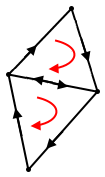
\includegraphics[scale=0.7]{images/c11.2.png}
    \caption{Согласованная ориентация треугольников триангуляции.}
    \label{fig:c11.2}
\end{figure}

Такие треугольники (см.рис.\ref{fig:c11.2}) будем называть согласованно ориентированными.

\begin{definition}
    Многообразие называется \textit{ориентируемым}, если на треугольниках его триангуляции можно ввести согласованную ориентацию.
\end{definition} 

\begin{statement}
    Свойство поверхности двумерного многообразия быть ориентируемым или неориентируемым не зависит от триангуляции.
\end{statement} 
\begin{proof}
    Без доказательства.
\end{proof} 

Пример неориентируемого многообразия: лист Мёбиуса (\ref{fig:mobius}). Это многообразие с краем. Зададим лист Мёбиуса в виде склейки прямоугольника и разобьём каким-либо образом этот прямоугольник на треугольники. После выбора на произвольном треугольнике направления обхода, на соседних треугольниках направление обхода границы задаётся однозначно. Как бы мы ни выбирали направление обхода при склейке листа Мёбиуса из прямоугольника по одной стороне, нам не удастся согласовать ориентацию на треугольниках, содержащих эту сторону.

Аналогичная ситуация в общем случае — выбрав направление обхода на одном треугольнике, мы однозначно ориентируем все остальные треугольники триангуляции (если поверхность связная). На плоскости (до склейки) это означает, что у всех треугольников будет направление обхода по или против часовой стрелки.

\begin{figure}[ht]
    \centering
    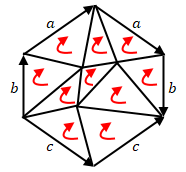
\includegraphics[scale=0.7]{images/c11.3.png}
    \caption{Задание ориентации поверхности.}
    \label{fig:c11.3}
\end{figure}

Несложно увидеть, что для всех сторон треугольников, находящихся внутри многоугольника, условие согласованности выполнено. Остаётся проверить (как и в случае с лентой Мёбиуса), согласована ли ориентация треугольников по сторонам многоугольника.

Отсюда следует, что понять, будет ли поверхность ориентируемой, можно по слову, которое её задаёт: если в слове есть пара одинаковых букв, встречающихся в одинаковых степенях, то задать ориентацию на поверхности не получится, а если все одинаковые буквы встречаются в разных степенях, то поверхность ориентируема.

Теперь можем дополнить классификацию: многообразия из первой и третьей серий ориентируемы, а из второй — неориентируемы.

\begin{statement}
    Двумерное многообразие неориентируемо тогда и только тогда, когда оно содержит лист Мёбиуса.
\end{statement} 


\subsubsection{Связные суммы и продолжение классификации}
\begin{definition}
    Пусть $M_1$ и $M_2$ — компактные связные двумерные многообразия. Вырежем диски в многообразии $M_1$ и в многообразии $M_2$ и полученные окружности в $M_1$ и $M_2$ склеим по какому-то гомеоморфизму. Получим новое многообразие $$M = M_1 \# M_2$$ — \textit{связная сумма многообразий $M_1$ и $M_2$}.
\end{definition} 

\begin{figure}[ht]
    \centering
    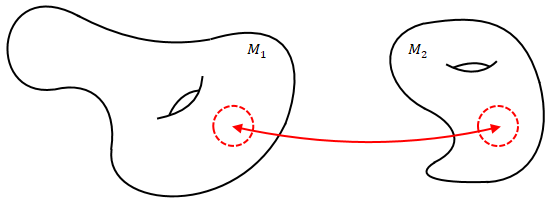
\includegraphics[scale=0.8]{images/c11.9.png}
    \caption{Связная сумма двух многообразий.}
    \label{fig:c11.9}
\end{figure}

Корректность определения: проверим, что после склейки получится двумерное многообразие (то есть, что после склейки окрестность каждой точки будет гомеоморфна двумерному диску). Окрестности точек, далёких от места склейки, не изменятся, нужно проверить, окрестности точек, которые принадлежат окружностям, по которым мы склеиваем многообразия: действительно, после склейки окрестности точек окружностей будут гомеоморфны двумерному диску. Также необходимо проверить, что результат операции не зависит от выбора вырезаемых дисков.

\begin{theorem}
    Любое связное компактное двумерное многообразие гомеоморфно одному из следующих:
    \begin{enumerate}
        \item $\mathbb{S}^2$;
        \item $\mathbb{T} \# \dots \# \mathbb{T}$, где $\mathbb{T}$ — тор;
        \item $\mathbb{RP}^2 \# \dots \# \mathbb{RP}^2$.
    \end{enumerate}
\end{theorem} 
\begin{proof}
    \begin{remark}
        Для любого двумерного многообразия $X$ выполнено
        \[X \# \mathbb{S}^2 = M,\]
        поэтому можно сказать, что любое связное компактное двумерное многообразие гомеоморфно одному из следующих:
        \begin{enumerate}
            \item $\mathbb{T} \# \dots \# \mathbb{T} \# \mathbb{S}^2$
            \item $\mathbb{RP}^2 \# \dots \# \mathbb{RP}^2$.
        \end{enumerate}
    \end{remark}

    Рассмотрим процесс взятия связной суммы для многообразий, представленных в виде склейки многоугольников. Пример (два тора, склеенных из квадрата):

    \begin{figure}[ht]
        \centering
        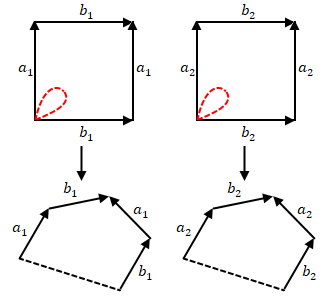
\includegraphics[scale=0.7]{images/c11.4.png}
        \caption{Вырезание диска в торе.}
        \label{fig:c11.4}
    \end{figure}

    Поскольку результат взятия связной суммы не зависит от того, где мы вырежем диск, вырежем его так, как показано на рисунке \ref{fig:c11.4} (пунктиром отмечена граница, которая получалась после вырезания диска). Склеив стороны, отмеченные пунктиром получим восьмиугольник (см.рис.\ref{fig:c11.5}).

    \begin{figure}[ht]
        \centering
        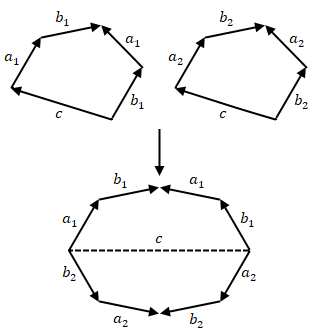
\includegraphics[scale=0.7]{images/c11.5.png}
        \caption{Склейка квадратов с вырезанным диском.}
        \label{fig:c11.5}
    \end{figure}

    Иными словами, связная сумма $\mathbb{T}^2 \# \mathbb{T}^2$ получается как результат склейки такого восьмиугольника. То есть, слова $a_1 b_1 a_1^{-1} b_1^{-1}$ и $a_2 b_2 a_2^{-1} b_2^{-1}$ склеиваются в слово $a_1 b_1 a_1^{-1} b_1^{-1} a_2 b_2 a_2^{-1} b_2^{-1}$.

    Для произвольных двух слов рассуждения совершенно аналогичные — если есть многоугольники $W_1 = a_i b_k \dots$ и $W_2 = c_j d_l \dots$, то, вырезая таким образом диски и склеивая многоугольники по границе получившихся разрезов, получим, что многообразие, которое будет соответствовать связной сумме $M_1 \# M_2$, будет задаваться словом $W_1 W_2$, которое получается приписыванием к слову $W_1$ слова $W_2$.

    Тогда в первой серии слово состоит из четвёрок букв, где каждая четвёрка задаёт тор, а во второй серии слово состоит из пар букв, где каждая пара задаёт проективную плоскость.

    Как и в примере с тором, для взятия связной суммы неориентируемых многообразий, вырезаем диск, как показано на рисунке (\ref{fig:c11.6}).

    \begin{figure}[ht]
        \centering
        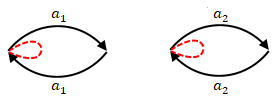
\includegraphics[scale=0.7]{images/c11.6.png}
        \caption{Склейка проективных плоскостей.}
        \label{fig:c11.6}
    \end{figure}

    На языке связных сумм можно пояснить некоторые названия, которые принято приписывать многообразиям из тех серий, которые мы получили.

    Процесс взятия связной суммы с тором обычно называют приклейкой ручки. Название для многообразий из первой серии теоремы классификаций — это сфера с $n$ ручками (каждая ручка — операция взятия связной суммы с тором).

    \begin{figure}[ht]
        \centering
        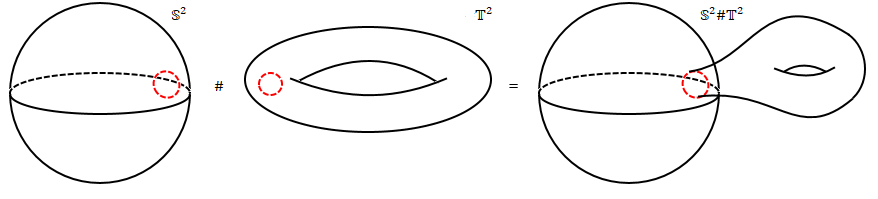
\includegraphics[scale=0.5]{images/c11.7.png}
        \caption{Связная сумма многообразия с тором.}
        \label{fig:c11.7}
    \end{figure}

    Многообразия из второй серии теоремы классификации называют сферой с $m$ плёнками Мёбиуса. На примере сферы посмотрим, что происходит при взятии связной суммы многообразия с проективной плоскостью (будем для проективной плоскости использовать модель диска, у которого отождествлены диаметрально противоположные точки на границе).

    Вырежем диски на проективной плоскости и на сфере. Проективная плоскость — это объединение листа Мёбиуса с диском $D^2$.

    \begin{figure}[htbp]
        \centering
        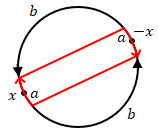
\includegraphics[scale=0.7]{images/c11.8.png}
        \caption{Проективная плоскость — объединение диска и листа Мёбиуса.}
        \label{fig:c11.8}
    \end{figure}

    То есть, можно разрезать проективную плоскость замкнутой кривой (выделена красным на рисунке (\ref{fig:c11.8})) на диск и лист Мёбиуса. Поэтому связная сумма сферы с проективной плоскостью — это приклейка листа Мёбиуса к сфере.

    Итак, любое связное компактное двумерное многообразие гомеоморфно либо сфере с $n$ ручками, либо сфере с $m$ плёнками Мёбиуса.
\end{proof} 